\documentclass[11pt]{article}
\usepackage[margin=2.2cm]{geometry}
\usepackage{fontspec}
\usepackage{graphicx}
\usepackage{booktabs}
\usepackage{tabularx}
\usepackage{xcolor}
\usepackage{listings}
\usepackage{tikz}
\usetikzlibrary{positioning,arrows.meta}
\usepackage[hidelinks]{hyperref}
\usepackage{enumitem}

\setlist{itemsep=2pt,topsep=4pt}
\definecolor{codeback}{gray}{0.96}
\definecolor{codekeyword}{RGB}{0,70,160}
\definecolor{codecomment}{RGB}{90,120,70}
\lstset{
	language=C++,
	basicstyle=\ttfamily\small,
	keywordstyle=\color{codekeyword},
	commentstyle=\color{codecomment},
	backgroundcolor=\color{codeback},
	frame=none,
	xleftmargin=0.6em,
	framexleftmargin=0.6em,
	aboveskip=8pt,
	belowskip=8pt,
	tabsize=4,
	columns=fullflexible,
	keepspaces=true,
	showstringspaces=false
}

\title{\textbf{litefont}\\[2pt]\large A small font engine for OpenGL and the CPU}
\author{Shane Transue}
\date{}

\begin{document}
\sloppy
\maketitle

\section{Overview}

litefont turns OpenType fonts into crisp text. It reads the font file itself, renders hinted glyph images with exact antialiasing, lays out paragraphs and labels, and draws them through OpenGL (1.1 fixed function or a 3.3 core profile) or into an image on the CPU. It is written in C++20, depends only on the standard library and the system's OpenGL, and needs no extension loader: it finds the OpenGL functions it uses by itself.

\begin{itemize}
	\item \textbf{Fonts:} TrueType and CFF (\texttt{.otf}) outlines, collections (\texttt{.ttc}), kerning from GPOS or the kern table, names and traits; damaged files fail cleanly.
	\item \textbf{Families:} regular, bold, italic and bold italic faces, simulated when missing; fallback families for missing code points; a catalog that finds families by name in a folder.
	\item \textbf{Glyphs:} exact-area coverage with vertical hinting; outlines, sharp and blurred shadows, all cached in a texture atlas; gradients with a color in each corner.
	\item \textbf{Layout:} wrapping, alignment, tabs, letter spacing, line limits with an ellipsis, superscripts and subscripts, underline and strikethrough, per-range colors and styles, anchors and quarter-turn rotation.
	\item \textbf{Editing queries:} caret boxes, selection rectangles, hit tests and caret movement.
\end{itemize}

\begin{figure}[h]
	\centering
	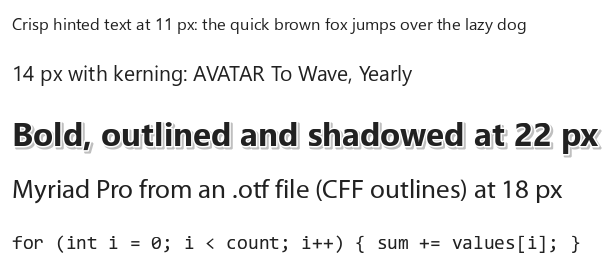
\includegraphics[width=0.78\textwidth]{figures/samples.png}
	\caption{Text drawn by litefont on the CPU at 150 percent scale: hinted small text, kerning, a bold outlined and shadowed label, a CFF font and monospaced code.}
\end{figure}

\section{Quick start}

A program declares a font, a device for its kind of OpenGL context and a renderer, loads the font once, and draws wherever it already draws. Neither the device nor the renderer needs an OpenGL context until the first draw.

\begin{lstlisting}
#include <litefont/litefont.h>

litefont::Font font;                       // (1) declare
litefont::OpenGL11Device device;           // or OpenGL33Device
litefont::OpenGLRenderer renderer(device);

void init() {
	font.load("DejaVuSans.ttf");           // (2) load once
}

void display() {
	glBegin(GL_TRIANGLES);                 // the program's own drawing
	// ...
	glEnd();
	renderer.drawText(font, 16.0f, "Hello world", 20.0f, 40.0f);   // (3) draw
}
\end{lstlisting}

Positions are pixels from the top-left corner of the viewport. \texttt{measureText} gives the box a string takes, for centering or right alignment, and \texttt{setScale} sets the device pixels per pixel on high-density screens.

\section{How it works}

\begin{center}
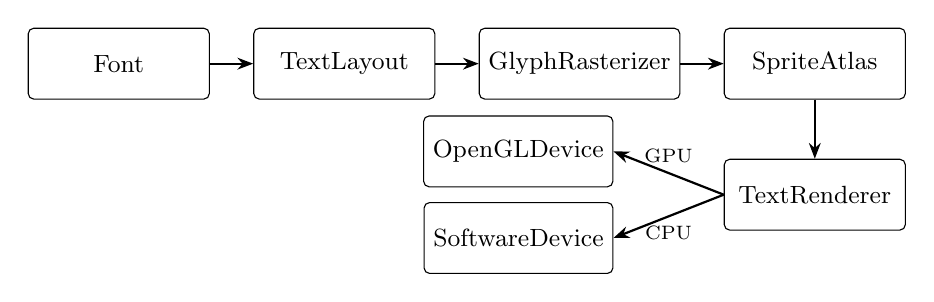
\begin{tikzpicture}[
	stage/.style={draw, rounded corners=2pt, minimum height=0.9cm, minimum width=2.3cm, align=center, font=\small},
	arrow/.style={-{Stealth[length=2mm]}, thick}]
	\node[stage] (font) {Font};
	\node[stage, right=0.55cm of font] (layout) {TextLayout};
	\node[stage, right=0.55cm of layout] (glyphs) {GlyphRasterizer};
	\node[stage, right=0.55cm of glyphs] (atlas) {SpriteAtlas};
	\node[stage, below=0.75cm of atlas] (renderer) {TextRenderer};
	\node[stage, left=1.4cm of renderer, yshift=0.55cm] (opengl) {OpenGLDevice};
	\node[stage, left=1.4cm of renderer, yshift=-0.55cm] (software) {SoftwareDevice};
	\draw[arrow] (font) -- (layout);
	\draw[arrow] (layout) -- (glyphs);
	\draw[arrow] (glyphs) -- (atlas);
	\draw[arrow] (atlas) -- (renderer);
	\draw[arrow] (renderer.west) -- (opengl.east) node[midway, above, font=\scriptsize] {GPU};
	\draw[arrow] (renderer.west) -- (software.east) node[midway, below, font=\scriptsize] {CPU};
\end{tikzpicture}
\end{center}

A \textbf{Font} owns its file's bytes and answers questions about them: metrics, the glyph for a code point, advances, kerning and outlines. \textbf{TextLayout} places the glyphs of a \textbf{Text} (its content, family, size, colors and layout settings) on whole-pixel baselines. The \textbf{GlyphRasterizer} renders each glyph at its size, hinted so baselines and x-heights land on whole pixels, and the \textbf{SpriteAtlas} keeps the images in texture pages. The \textbf{TextRenderer} turns placed glyphs into quads and hands them to a \textbf{GraphicsDevice}: an \textbf{OpenGLDevice} (OpenGL11Device or OpenGL33Device) on the GPU or \textbf{SoftwareDevice} on the CPU, which use the same blending and give the same pixels to within one level.

A Text is laid out once and kept. Drawing it again, or moving it, costs no layout and no glyph rendering; only a change to how it looks starts over.

\section{Drawing with OpenGL}

\texttt{OpenGLRenderer} is the immediate-mode front end. Each \texttt{drawText} call draws at once, in call order with the program's own drawing. Behind it, every distinct string with its font, size, style and color keeps its layout and glyphs, so a string drawn every frame, even at a new position, costs a lookup and moving its quads. The least recently drawn strings are dropped once the cache holds more than 1024. \texttt{draw(text, x, y)} does the same for a Text with all its own settings.

The renderer draws through the device the program picked for its context:
\begin{itemize}
	\item \texttt{OpenGL11Device} uses only OpenGL 1.1 fixed function, so it runs in any compatibility context, next to \texttt{glBegin} and \texttt{glEnd}. Glyph pages are alpha textures, modulated by the vertex color and blended with straight alpha. It saves and restores the program's state with \texttt{glPushAttrib}, \texttt{glPushClientAttrib} and the matrix stacks.
	\item \texttt{OpenGL33Device} runs in 3.3 or newer contexts, core profiles included. It draws with one small shader from a vertex array and buffers; glyph pages are one-channel textures read as alpha, so it blends exactly as the 1.1 device does. Core profiles have no attribute stack, so it reads each value it changes and sets it back afterwards.
\end{itemize}
For each draw a device sets what text needs (a projection, blending, the atlas texture, the scissor for clips) and switches off depth test and face culling. \texttt{setRestoreState(false)} skips saving and restoring for programs that manage their own state.

Neither device includes an OpenGL header or needs a loader. Each finds its functions at the first draw through a table of them (\texttt{OpenGL11Functions}, \texttt{OpenGL33Functions}); \texttt{OpenGLFunctions.cpp} is the only file that knows the operating system, and looks functions up with \texttt{wglGetProcAddress} on Windows, in the OpenGL framework on macOS, and through EGL or GLX on Linux. Textures, buffers and the shader are made at the first draw too; \texttt{release()} deletes them while the context is current, and \texttt{getError()} says why a device drew nothing.

\subsection*{Text in the program's own transform}

By default text sits on the pixel grid of the viewport. To draw it in the program's own coordinates instead, such as a zoomable 2D view, a turning label or a point in a 3D scene, the program tells the device: \texttt{setMatrix(m)} takes a column-major matrix (projection times model-view, as a shader would), and on \texttt{OpenGL11Device}, \texttt{useMatrixStack()} draws through whatever the program set with \texttt{glOrtho}, \texttt{glRotatef} and the rest. \texttt{useViewport()} goes back to pixels.

\begin{lstlisting}
glMatrixMode(GL_MODELVIEW);
glRotatef(degrees, 0.0f, 0.0f, 1.0f);
device.useMatrixStack();
renderer.draw(label);
device.useViewport();
\end{lstlisting}

Positions and sizes are then in the program's units, and text grows downward from its position; y is up by default, and \texttt{setYUp(false)} serves a y-down space. Each string is rendered at about the size it covers on screen, in steps of a sixth of an octave, and the matrix carries it the rest of the way with linear filtering, so text stays sharp at any zoom, and moving, turning or zooming it costs no new layout until its size crosses a step.

\section{Texts and labels}

A \texttt{Text} holds everything about how a piece of text looks. Changing a setting marks it for a new layout, except the offset and clip, which only move or cut what is drawn.

\begin{center}
\small
\begin{tabularx}{\textwidth}{@{}lX@{}}
\toprule
Setting & Effect \\
\midrule
content, family, size & UTF-8 text, the faces it uses, its size in pixels \\
style, style runs & a face per range of bytes, superscript or subscript, underline, strikethrough \\
color, color runs & a color per range of bytes, such as syntax colors \\
gradient & a color for each corner of the box, blended across the glyphs \\
outline, shadow & a border around each glyph; an offset shadow, optionally blurred \\
background & a box behind the text, grown by padding \\
max width, align, line spacing, tab width & paragraph layout \\
letter spacing, max lines, ellipsis & spacing between glyphs; cutting long text with an ellipsis \\
anchor, rotation & the point of the box that lands on the position; a quarter turn \\
offset, clip & where it is drawn and what it may cover, with no new layout \\
\bottomrule
\end{tabularx}
\end{center}

\texttt{TextCursor} answers the geometry an editor needs from a layout: the caret box, selection rectangles, the position a point hits, and where the caret moves by character, word or line.

\section{Fonts}

A \texttt{Font} loads a \texttt{.ttf}, \texttt{.otf} or one face of a \texttt{.ttc} file, from a path or from bytes in memory. A \texttt{FontFamily} groups up to four faces and simulates bold and italic where a face is missing; fallback families supply code points the family lacks, and the replacement character marks those nobody has. A \texttt{FontCatalog} reads only the names and traits of the fonts in a folder, from a few small reads per file, and loads a family by name. litefont never looks for system fonts by itself: it reads the files and folders a program names.

\section{Building}

litefont builds with CMake 3.20 or newer and any C++20 compiler.
\begin{lstlisting}[language=bash]
cmake -S . -B build
cmake --build build --config Release
\end{lstlisting}
\texttt{LITEFONT\_BUILD\_EXAMPLES} adds the freeglut example and a command-line renderer, \texttt{LITEFONT\_BUILD\_TESTS} the test suite, and \texttt{LITEFONT\_OPENGL} can turn the OpenGL renderers off for CPU-only use. A project adds litefont with \texttt{add\_subdirectory}, or installs it and uses \texttt{find\_package(litefont)}; either way it links \texttt{litefont::litefont}.

\end{document}
